% Options for packages loaded elsewhere
\PassOptionsToPackage{unicode}{hyperref}
\PassOptionsToPackage{hyphens}{url}
%
\documentclass[
]{article}
\usepackage{amsmath,amssymb}
\usepackage{lmodern}
\usepackage{ifxetex,ifluatex}
\ifnum 0\ifxetex 1\fi\ifluatex 1\fi=0 % if pdftex
  \usepackage[T1]{fontenc}
  \usepackage[utf8]{inputenc}
  \usepackage{textcomp} % provide euro and other symbols
\else % if luatex or xetex
  \usepackage{unicode-math}
  \defaultfontfeatures{Scale=MatchLowercase}
  \defaultfontfeatures[\rmfamily]{Ligatures=TeX,Scale=1}
\fi
% Use upquote if available, for straight quotes in verbatim environments
\IfFileExists{upquote.sty}{\usepackage{upquote}}{}
\IfFileExists{microtype.sty}{% use microtype if available
  \usepackage[]{microtype}
  \UseMicrotypeSet[protrusion]{basicmath} % disable protrusion for tt fonts
}{}
\makeatletter
\@ifundefined{KOMAClassName}{% if non-KOMA class
  \IfFileExists{parskip.sty}{%
    \usepackage{parskip}
  }{% else
    \setlength{\parindent}{0pt}
    \setlength{\parskip}{6pt plus 2pt minus 1pt}}
}{% if KOMA class
  \KOMAoptions{parskip=half}}
\makeatother
\usepackage{xcolor}
\IfFileExists{xurl.sty}{\usepackage{xurl}}{} % add URL line breaks if available
\IfFileExists{bookmark.sty}{\usepackage{bookmark}}{\usepackage{hyperref}}
\hypersetup{
  pdftitle={Multilevel Regression Modeling as a Complement to Traditional Repeated Measures Analysis of Variance in Sports Biomechanics Research},
  hidelinks,
  pdfcreator={LaTeX via pandoc}}
\urlstyle{same} % disable monospaced font for URLs
\usepackage[margin=1in]{geometry}
\usepackage{longtable,booktabs,array}
\usepackage{calc} % for calculating minipage widths
% Correct order of tables after \paragraph or \subparagraph
\usepackage{etoolbox}
\makeatletter
\patchcmd\longtable{\par}{\if@noskipsec\mbox{}\fi\par}{}{}
\makeatother
% Allow footnotes in longtable head/foot
\IfFileExists{footnotehyper.sty}{\usepackage{footnotehyper}}{\usepackage{footnote}}
\makesavenoteenv{longtable}
\usepackage{graphicx}
\makeatletter
\def\maxwidth{\ifdim\Gin@nat@width>\linewidth\linewidth\else\Gin@nat@width\fi}
\def\maxheight{\ifdim\Gin@nat@height>\textheight\textheight\else\Gin@nat@height\fi}
\makeatother
% Scale images if necessary, so that they will not overflow the page
% margins by default, and it is still possible to overwrite the defaults
% using explicit options in \includegraphics[width, height, ...]{}
\setkeys{Gin}{width=\maxwidth,height=\maxheight,keepaspectratio}
% Set default figure placement to htbp
\makeatletter
\def\fps@figure{htbp}
\makeatother
\setlength{\emergencystretch}{3em} % prevent overfull lines
\providecommand{\tightlist}{%
  \setlength{\itemsep}{0pt}\setlength{\parskip}{0pt}}
\setcounter{secnumdepth}{5}
\usepackage{authblk}
\usepackage{array}
\usepackage{color,soul}
\usepackage{setspace}
\usepackage{etoolbox,lineno}
\usepackage{amsmath}
\usepackage{mathtools}
\usepackage{threeparttable}
\usepackage{tabularx}
\usepackage{hhline}
\usepackage{booktabs}
\usepackage{float}
\usepackage{caption}
\usepackage{array,multirow}
\usepackage[superscript]{cite}
\usepackage[acronym,toc,nonumberlist]{glossaries}
\usepackage[small]{titlesec}
\usepackage[none]{hyphenat}
\renewcommand*{\contentsname}{Table of Contents}
\renewcommand{\thefootnote}{\roman{footnote}}
\setlength{\parindent}{0.375in}
\author[1,2]{\footnotesize Kyle Wasserberger}
\author[3]{\footnotesize William Murrah}
\author[4]{\footnotesize Kevin Giordano}
\author[2]{\footnotesize Gretchen Oliver}
\affil[1]{Research \& Development; Driveline Baseball}
\affil[2]{School of Kinesiology; Auburn University}
\affil[3]{\footnotesize Department of Educational Foundations, Leadership, \& Technology; Auburn University}
\affil[4]{\footnotesize Department of Physical Therapy; Creighton University}
\newcolumntype{L}[1]{>{\small\raggedright\let\newline\\\arraybackslash\hspace{-1pt}}p{#1}}
\newcolumntype{C}[1]{>{\small\centering\let\newline\\\arraybackslash\hspace{-1pt}}p{#1}}
\newcolumntype{R}[1]{>{\small\raggedleft\let\newline\\\arraybackslash\hspace{-1pt}}p{#1}}
\ifluatex
  \usepackage{selnolig}  % disable illegal ligatures
\fi

\title{Multilevel Regression Modeling as a Complement to Traditional Repeated Measures Analysis of Variance in Sports Biomechanics Research}
\date{\vspace{-2.5em}}

\begin{document}
\maketitle

\pagenumbering{gobble}
\begin{center}
Keywords: mixed-effects, hierarchical, longitudinal, growth curve
\end{center}

\newpage
\linenumbers
\begin{abstract}
\doublespacing
With the growing availability of sport science technologies, longitudinal data are becoming increasingly available to the biomechanics and broader sport science communities. To take full advantage of this emerging wealth of data and understand  its impact on injury and performance research, considerations regarding the appropriate handling of longitudinal data are needed. Traditionally, longitudinal data have been analyzed using repeated measures analysis of variance (RM $\cdot$ ANOVA). However, RM $\cdot$ ANOVA is limited in its ability to handle missing data and unbalanced designs, two scenarios common in longitudinal studies. Alternatively, multilevel regression modeling is a flexible yet neglected analysis method in the sports biomechanics literature but capable of handling unbalanced designs and missing data (among other benefits). In this paper, we hope to draw increased attention to this underused research tool and lobby for its increased adaptation when examining repeated measures biomechanics data. First, we introduce the rationale and approach underlying multilevel regression models. We then present examples using simulated and real-world data to illustrate their potential application and limitations in sports biomechanics research. Lastly, we provide some recommendations, words of caution, and additional resources.
\end{abstract}

\newpage
\pagenumbering{arabic}

\hypertarget{introduction}{%
\section{Introduction}\label{introduction}}

\doublespacing

We biomechanists like to throw away lots of data. Our cameras capture the positions of dozens of reflective markers with sub-millimeter accuracy hundreds of times each second while our participants perform several, sometimes dozens, of movement trials during data collection. Each new trial brings additional data that could increase statistical power and be used to better understand our research questions. Yet, far too often, choices related to experimental design or statistical analysis greatly reduce the volume of data we work with. Reduced data volume negatively impacts inferential power when conducting statistical analyses and can potentially indicate inefficient use of data collection resources and research labor.

Two research practices common in sports biomechanics that reduce data volume are discretization and ensemble averaging. Discretization occurs when researchers extract one value, such as a maxima, minima, or average value, from a continuous time series of data. Ensemble averaging occurs when researchers combine several trials from the same participant into one \emph{representative} trial. Discretization and ensemble averaging can also be combined to further reduce the available data by averaging discrete values from multiple trials or taking discrete values from ensemble averaged time series. Although sometimes appropriate depending on the research question, discretization and ensemble averaging reduce the dimensionality and variability in time series data, reducing statistical power.

While discretization can be ameliorated though emerging techniques such as statistical parametric mapping \cite{pataky2019}, researchers may still wish to examine certain discrete measures if warranted by their domain expertise and research question of interest. One such scenario is the repeated measure of biomechanic or performance values over time. Typically, repeated measures data in sports biomechanics are examined using univariate or multivariate repeated measures analysis of (co)variance. While these statistical tools are appropriate under certain conditions, they make several assumptions that may often be problematic in the observational or quasi-experimental settings common in sport biomechanics research. In such cases, multilevel regression modeling may complement or replace more traditional repeated measures analyses.

Although multilevel techniques are present in other sport performance domains such as sport psychology \cite{beauchamp2005,benson2016,cornelius2007}, they have yet to make significant headway into sport biomechanics. If fact, to our knowledge, the use of multilevel modeling in sport biomechanics is limited to two papers, both published since 2019 \cite{slowik2019, iglesias2021}. Slowik et. al.~used a multilevel framework to contrast the strong within and weak between-participant relationships between elbow joint loading and baseball pitching speed \cite{slowik2019} while Iglesias et. al.~examined between-participant differences in the within-participant load-velocity relationship during several weightlifting exercises \cite{iglesias2021}. Although these two papers provide important insight into their respective research areas, we feel a formal introduction of the advantages, disadvantages, and limitations of multilevel modeling would benefit those in sport biomechanics working with repeated measures designs. Therefore, our purpose is to introduce multilevel regression modeling to a sports biomechanics audience and offer a brief tutorial on model notation, construction, and interpretation. We also outline the advantages and disadvantages of multilevel modeling over traditional repeated measures designs and offer recommendations for those interested in further exploration of multilevel techniques.

\hypertarget{the-traditional-regression-model}{%
\section{The Traditional Regression Model}\label{the-traditional-regression-model}}

Before examining the multilevel regression model, let us first consider a simple linear regression predicting some outcome measure, \(y\), from one predictor variable, \(x\), given by Equation \ref{eq:reg1}:

\begin{equation}
\hat{y}_{i}=\beta_{0}+\beta_{1}x_{i}+\epsilon_{i}
\label{eq:reg1}
\end{equation}

\noindent
In Equation \ref{eq:reg1}, \(\beta_{0}\) represents the model intercept and \(\beta_{1}\) represents the model slope. Recall that a model intercept can be thought of as the predicted value of \(y\) when \(x\) equals zero and a model slope can be thought of as the predicted increase (or decrease, if negative) in \(y\) for a 1-unit increase in \(x\). \(\epsilon_{i}\) represents the residual error between the \(i\)-th model prediction and the \(i\)-th observed data point (\(y_{i}-\hat{y}_{i}\)) (Figure \ref{fig1}). The one-predictor linear regression model can be extended to multiple regression by adding additional predictor variables (i.e.~\(x_{2}\), \(x_{3}...x_{n}\)) or non-linear regression by adding polynomial (i.e.~\(x^{2}, x^{3}...x^{n}\)), exponential (\(e^{x}\)), or logarithmic (\(ln(x)\)) terms. Additionally, how predictor variables' effects depend on one another can be examined by introducing their product terms (i.e.~\(x_{1}*x_{2}\)) and analyzing their interactions.

\begin{figure}[H]
\centering
\captionsetup{width=0.6\textwidth}
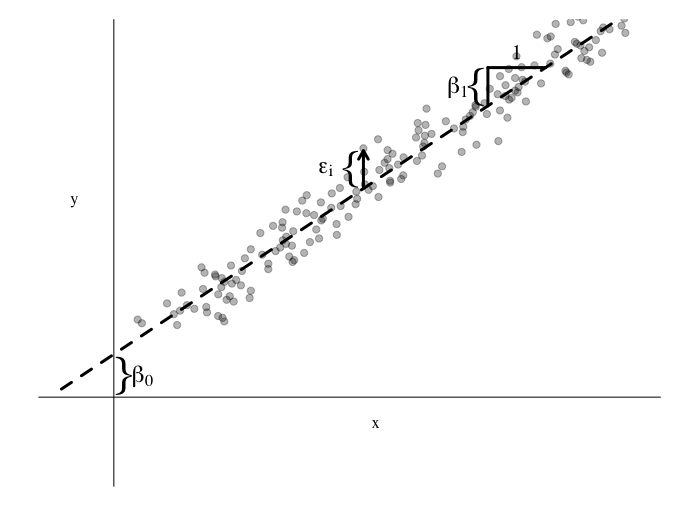
\includegraphics[width=0.6\textwidth]{fig1.png}
\caption{Hypothetical Simple Regression}
\label{fig1}
\end{figure}

\hypertarget{the-multilevel-regression-model-for-repeated-measures}{%
\section{The Multilevel Regression Model for Repeated Measures}\label{the-multilevel-regression-model-for-repeated-measures}}

Similar to traditional regression, we can start with a simple multilevel model predicting some outcome measure, \(y\), from one predictor variable, \(x\). For this paper we will be following Hox's \cite{hox2017} notation\footnote{It should be known that other authors have used slightly (or sometimes very) different notations. Admittedly, this is one of the higher barriers to entry for those without strong analytical training. We encourage readers to take considerable time learning model notation as it will accelerate the remaining stages of the learning process}.

\begin{equation}
\hat{y}_{ij}=\beta_{0j}+\beta_{1j}x_{ij}+\epsilon_{ij}
\label{eq:mlm1}
\end{equation}

\noindent
Equation \ref{eq:mlm1} is often referred to as the \emph{level-one} or \emph{first-level} model since it deals with the first level of nesting in our data. In repeated measures designs, observations are nested within individuals so we consider observations to be at the first, or lower, level and individuals to be at the second, or higher, level. In other applications, multilevel models may have individuals at the first level nested within some grouping structure such as classrooms, congressional districts, or treatment arms.

Equation \ref{eq:mlm1} is identical to Equation \ref{eq:reg1} except we now have a second subscript, \(j\), denoting the nested nature of the data. \(x_{ij}\) now represents the \(i\)-th observation from the \(j\)-th individual while \(\beta_{0j}\) and \(\beta_{1j}\) represent the \(j\)-th individual's model intercept and slope. \(\hat{y}_{ij}\) represents the model prediction for the \(i\)-th observation from the \(j\)-th individual and \(\epsilon_{ij}\) represents the residual error between each observed outcome and its corresponding predicted value (\(y_{ij}-\hat{y}_{ij}\)). The inclusion of a second subscript, \(j\), thereby allowing model intercepts and slopes to vary between individuals is the fundamental difference between traditional and multilevel regression.

By allowing model intercepts and slopes to vary between individuals, the multilevel model for repeated measures parses each individual's intercept and slope into a combination of the average model intercept/slope plus some individual-specific deviation from the average. Equations \ref{eq:mlm_int} and \ref{eq:mlm_slope} represent the regression equations predicting each individual's model intercept (Equation \ref{eq:mlm_int}) and slope (Equation \ref{eq:mlm_slope}) and make up the second-level model. In Equations \ref{eq:mlm_int} and \ref{eq:mlm_slope} the first term on the right side (\(\gamma_{00}\) and \(\gamma_{10}\)) represent the \emph{average} model intercept and slope, respectively. These average model parameters are known as \emph{fixed}-effects since they do not vary between individuals (notice there is no \(j\) subscript). The second terms on the right side (\(\mu_{0j}\) and \(\mu_{1j}\)) represent the individual-specific deviations from the average model intercept and slope, respectively. Because \(\mu_{0j}\) and \(\mu_{1j}\) vary between individuals, they are known as \emph{random}-effects. Modeling parameter variability as a combination of fixed and random-effects is why multilevel models are sometimes referred to as \emph{mixed}-effects models (a mixture of fixed and random effects).

\begin{align}
\beta_{0j}&=\gamma_{00}+\mu_{0j}\label{eq:mlm_int}\\
\beta_{1j}&=\gamma_{10}+\mu_{1j}\label{eq:mlm_slope}
\end{align}

\noindent
The multilevel model can then use second-level parameters (\(z_{j}\)) to account for variance in the predicted intercepts and slopes. With the inclusion of second-level parameters, \(\mu_{0j}\) and \(\mu_{1j}\) represent the residual variation in the predicted intercept and slope after accounting for \(z_{j}\).

\begin{align}
\beta_{0j}&=\gamma_{00}+\gamma_{01}z_{j}+\mu_{0j}\label{eq:mlm_int_full}\\
\beta_{1j}&=\gamma_{10}+\gamma_{11}z_{j}+\mu_{1j}\label{eq:mlm_slope_full}
\end{align}

\noindent
Substituting the right side of Equations \ref{eq:mlm_int_full} and \ref{eq:mlm_slope_full} for \(\beta_{0j}\) and \(\beta_{1j}\) from Equation \ref{eq:mlm1} yields the complete multilevel model predicting one outcome from one first-level and one second-level variable:

\begin{equation}
\hat{y}_{ij}=\overbrace{\textstyle \gamma_{00}+\gamma_{01}z_{j}+\mu_{0j}}^{\mathclap{intercept}}+
\overbrace{\textstyle (\gamma_{10}+\gamma_{11}z_{j}+\mu_{1j})}^{\mathclap{slope}}x_{ij}+\epsilon_{ij}
\label{eq:mlm2}
\end{equation}

\noindent
Distributing \(x_{ij}\) and arranging like terms helps delineate the fixed and random parts of the model:

\begin{equation}
\hat{y}_{ij}=\overbrace{\textstyle 
\gamma_{00}+\gamma_{01}z_{j}+\gamma_{10}x_{ij}+\gamma_{11}x_{ij}z_{j}}^{\mathclap{fixed}}+
\overbrace{\textstyle \mu_{1j}x_{ij}+\mu_{0j}+\epsilon_{ij}}^{\mathclap{random}}
\label{eq:mlm3}
\end{equation}

\noindent
As with traditional regression models, the multilevel regression model can be generalized to multiple multilevel\footnote{yeah, "multiple multilevel", I know. Yikes} regression with \(m\) first-level and \(n\) second-level predictors:

\begin{align}
\hat{y}_{ij}=&\beta_{0j}+\sum\limits_{m=1}^{m}\beta_{mj}x_{mij}+\epsilon_{ij}\\
\beta_{0j}=&\gamma_{00}+\sum\limits_{n=1}^{n}\gamma_{0n}z_{nj}+\mu_{0j}\\
\beta_{mj}=&\gamma_{m0}+\sum\limits_{n=1}^{n}\gamma_{1n}z_{nj}+\mu_{nj}
\label{eq:mlm4}
\end{align}

\hypertarget{benefits-and-drawbacks-of-multilevel-models-over-traditional-repeated-measures-anova}{%
\section{Benefits and Drawbacks of Multilevel Models over Traditional Repeated Measures ANOVA}\label{benefits-and-drawbacks-of-multilevel-models-over-traditional-repeated-measures-anova}}

The three assumptions made by repeated measures ANOVA that are most relevant to sport biomechanics: temporal equivalence, design balance, and case completeness.

\begin{table}[H]
\begin{threeparttable}
\begin{tabular}{L{0.25\textwidth}R{0.375\textwidth}R{0.375\textwidth}}
\toprule
& \multicolumn{1}{r}{Repeated Measures ANOVA} & \multicolumn{1}{r}{Multilevel Regression} \\
\cline{2-3}
Temporal equivalence\tnote{a} & Assumes repeated measures are equally spaced in time & Repeated measures may be unequally spaced in time \\ \hline
Balanced design & Assumes participants have same number of repeated measures & Participants may have different number of repeated measures \\ \hline
Case completeness & Assumes no missing data; incomplete cases are handled through listwise deletion & Missing data may be accounted for under certain circumstances\tnote{b} \\
\hhline{===}
\end{tabular}
\begin{tablenotes}[flushleft]
\scriptsize{
\item[a] "Temporal" equivalence does not only apply to growth models, where time is placed on the x-axis. It may be extended to "whatever is on the x-axis of your scatterplot".
\item[b] Missing data analysis is an extremely rich stand-alone area of research that we cannot do justice in this article alone. Readers are directed to works of Enders\cite{enders2010} for a more thorough exploration of the topic}
\end{tablenotes}
\end{threeparttable}
\end{table}

\hypertarget{when-anova-will-do-just-fine}{%
\subsection{When ANOVA will do just fine}\label{when-anova-will-do-just-fine}}

Simple pre-post designs with no missing data

\hypertarget{other-figures-to-incorporate}{%
\section{Other Figures to incorporate}\label{other-figures-to-incorporate}}

\begin{figure}[H]
\centering
\captionsetup{width=0.6\textwidth}
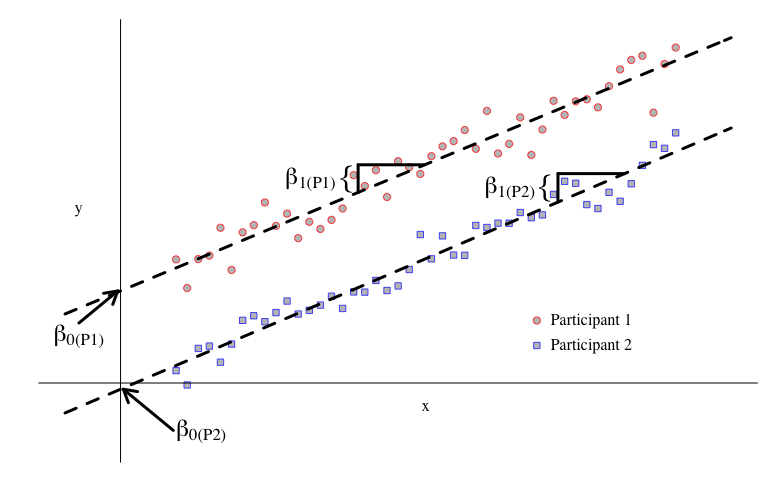
\includegraphics[width=0.6\textwidth]{rand_int.png}
\caption{Fictional multilevel model with random intercepts. Individual regression lines are parallel (equal slopes) but differ in their respective intercepts}
\label{fig-rand-int}
\end{figure}

\begin{figure}[H]
\centering
\captionsetup{width=0.6\textwidth}
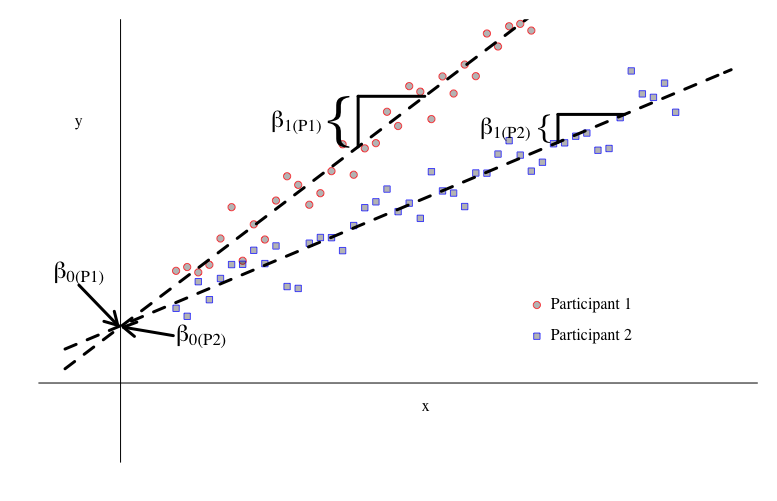
\includegraphics[width=0.6\textwidth]{rand_slope.png}
\caption{Fictional multilevel model with random slopes. Individual regression lines are not parallel (unequal slopes) but share a mutual intercept}
\label{fig-rand-slope}
\end{figure}

\begin{figure}[H]
\centering
\captionsetup{width=0.6\textwidth}
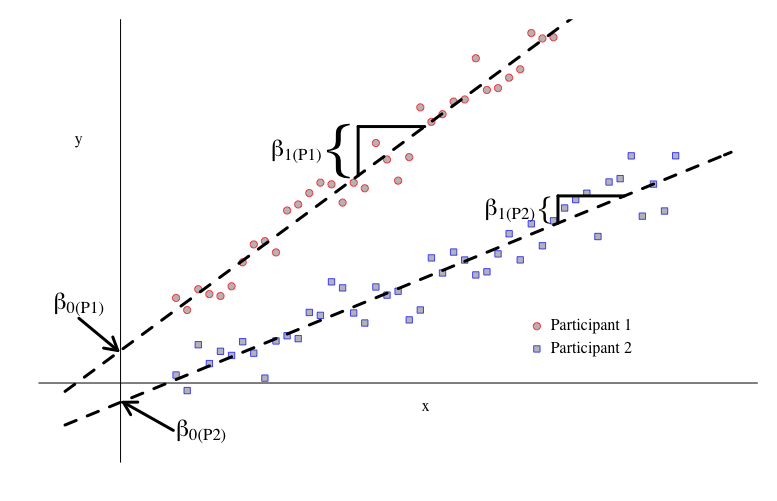
\includegraphics[width=0.6\textwidth]{rand_int_slope.png}
\caption{Fictional multilevel model with random intercepts and slopes. Individual regression lines are not parallel and do not share a mutual intercept}
\label{fig-rand-int-slope}
\end{figure}

\hypertarget{discard-pile}{%
\section{Discard Pile}\label{discard-pile}}

Some of the more notable assumptions that can cause problems for sport biomechanists dealing with repeated measures include temporal equivalence (i.e.~time between data points must be the same for all participants), balanced study designs (i.e.~must have the same number of data points for each individual) and case completeness (i.e.~must have no missing data).

Compared with traditional univariate or multivariate analysis of (co)variance, multilevel modeling allows more researcher flexibility through fewer statistical assumptions and the ability to handle missing data, non-linear relationships, and time-varying covariates \cite{hox2017}.

\newpage
\singlespacing
\addcontentsline{toc}{section}{References}
\bibliographystyle{plain-custom}
\bibliography{mlm_sport_biomech}

\end{document}
